% =============================================================================
% APPENDIX EVL: LIT-AUTHOR: Unknown Researcher Research Integration
% =============================================================================
% Category: LIT
% Language: English
% Version: 1.0 (January 2026)
% Status: Draft
%
% This appendix integrates research papers by Unknown Researcher into the EBF framework.
%
% =============================================================================

\chapter{LIT-AUTHOR: Unknown Researcher Research Integration}
\label{app:evl}

\begin{abstract}
This appendix integrates the research contributions of Unknown Researcher into the
Evidence-Based Framework. It documents key papers, core findings, and their
integration with EBF dimensions including complementarity parameters ($\gamma$),
context factors ($\Psi$), and utility dimensions.
\end{abstract}

\begin{tcolorbox}[colback=blue!5!white, colframe=blue!75!black,
    title=Quick Reference: Unknown Researcher Research]

\textbf{Appendix:} EVL (LIT)

\textbf{Researcher:} Unknown Researcher

\textbf{Core Themes:}
\begin{itemize}[nosep]
\item Behavioral economics foundations
\item Empirical evidence for EBF parameters
\item Policy implications and interventions
\end{itemize}

\textbf{EBF Integration:}
\begin{itemize}[nosep]
\item Complementarity values ($\gamma$) from experimental evidence
\item Context effects ($\Psi$) documented across studies
\item Utility dimension weightings calibrated to findings
\end{itemize}

\textbf{Cross-References:} BBB (CORE-WHERE), K (LIT-FEHR), G (Glossary)
\end{tcolorbox}

% -----------------------------------------------------------------------------
% APPENDIX SCOPE BOX
% -----------------------------------------------------------------------------

\begin{tcolorbox}[
    colback=orange!5!white,
    colframe=orange!75!black,
    title={\textbf{Appendix Scope: Ziel / In-Scope / Out-of-Scope / Constraints}},
    fonttitle=\bfseries
]

\textbf{Ziel (Objective):}
\begin{itemize}[nosep]
    \item Integrate Unknown Researcher's research into EBF with parameter extraction
\end{itemize}

\textbf{In-Scope:}
\begin{itemize}[nosep]
    \item Paper-by-paper integration with 10C mapping
    \item Extraction of $\gamma$, $\Psi$, and effect size parameters
    \item Cross-references to related EBF components
\end{itemize}

\textbf{Out-of-Scope (delegiert an andere Appendices):}
\begin{itemize}[nosep]
    \item Parameter validation $\rightarrow$ Appendix BBB (CORE-WHERE)
    \item Formal axiomatization $\rightarrow$ CORE appendices
    \item Meta-analysis $\rightarrow$ LIT-M appendices
\end{itemize}

\textbf{Constraints (Anwendungsgrenzen):}
\begin{itemize}[nosep]
    \item Parameters are extracted from published studies
    \item Effect sizes may vary across replications
    \item Context-specificity of findings applies
\end{itemize}

\textbf{Lieferobjekte (Deliverables):}
\begin{itemize}[nosep]
    \item Paper integration table with 10C mappings
    \item Extracted parameters for BBB repository
    \item Cross-reference map to related literature
\end{itemize}

\end{tcolorbox}



%%%%%%%%%%%%%%%%%%%%%%%%%%%%%%%%%%%%%%%%%%%%%%%%%%%%%%%%%%%%%%%%%%%%%%%%%%%%%%%
% APPENDIX R: Framework Evaluation Protocol
%%%%%%%%%%%%%%%%%%%%%%%%%%%%%%%%%%%%%%%%%%%%%%%%%%%%%%%%%%%%%%%%%%%%%%%%%%%%%%%
\section{Framework Evaluation Protocol}
\label{app:evaluationprotocol}

\paragraph{Abstract.}
This appendix establishes a standardized protocol for evaluating whether and
how academic papers contribute to the $(C, \Psi, C^*, K, Q)$ framework. The protocol 
provides: (1) a comprehensive checklist of dimensions to assess, (2) criteria
for distinguishing framework-supporting from framework-challenging evidence, (3)
a scoring system for evidential strength, and (4) a structured template for paper
analysis.

\subsection{Purpose and Scope}

\subsubsection{Why a Standardized Protocol?}

The $(C, \Psi, C^*, K, Q)$ framework claims to provide a unified lens for understanding 
economic behavior across diverse domains. To assess this claim rigorously, we need a 
systematic method for evaluating how individual papers relate to the framework. Without
such a method, we risk:

\begin{itemize}
  \item \textbf{Confirmation bias:} Selectively citing papers that support the framework
  \item \textbf{Vague integration:} Claiming papers ``fit'' without specifying how
  \item \textbf{Missed falsifications:} Overlooking evidence that challenges the framework
  \item \textbf{Inconsistent standards:} Applying different criteria to different papers
\end{itemize}

\subsubsection{What the Protocol Delivers}

For each paper analyzed, the protocol produces:
\begin{enumerate}
  \item \textbf{Framework Mapping:} Which framework elements does the paper address?
  \item \textbf{Contribution Classification:} Does it support, extend, qualify, or challenge the framework?
  \item \textbf{Evidence Assessment:} How strong is the evidential basis?
  \item \textbf{Integration Recommendation:} How should this paper be incorporated?
\end{enumerate}

\subsubsection{Framework Recap}

The framework consists of five core elements:
\begin{align}
  C &: \text{Complementarity matrix (interactions between choices/practices)} \\
  \Psi &: \text{Institutional/contextual parameters (culture, law, norms, networks)} \\
  C^* &: \text{Optimal configuration given } \Psi \\
  K &: \text{Knowledge/beliefs about } C \text{ and } \Psi \\
  Q &: \text{Outcomes (welfare, productivity, profits, utility)}
\end{align}

The central claims are:
\begin{itemize}
  \item Economic outcomes depend on complementarities ($C$) between choices
  \item Optimal configurations ($C^*$) depend on context ($\Psi$)
  \item Agents' knowledge ($K$) of $C$ and $\Psi$ affects behavior
  \item Outcomes ($Q$) reflect the alignment between actual choices and $C^*(\Psi)$
\end{itemize}

\subsection{The Evaluation Checklist}

\subsubsection{Part A: Basic Paper Information}

\begin{center}
\renewcommand{\arraystretch}{1.3}
\begin{tabular}{lp{10cm}}
\hline
\textbf{Item} & \textbf{Description} \\
\hline
A1. Citation & [Authors, Year, Title, Journal/Book] \\
A2. Field & [e.g., Organizational Economics, Labor, Development, Behavioral] \\
A3. Primary Question & [What question does the paper address?] \\
A4. Methodology & [Theory, Empirical-Observational, Experimental, Mixed] \\
A5. Data/Setting & [What data? Which context?] \\
\hline
\end{tabular}
\end{center}

\subsubsection{Part B: Framework Element Mapping}

For each framework element, assess whether and how the paper addresses it:

\paragraph{B1. Complementarity ($C$).}
\begin{itemize}
  \item Does the paper identify specific complementarities $C_{ij}$?
  \item What is the sign (positive/negative)?
  \item What is the mechanism?
  \item Is the complementarity tested empirically?
\end{itemize}

\paragraph{B2. Context ($\Psi$).}
\begin{itemize}
  \item Which $\Psi$ dimensions are addressed? (Technology, Institutions, Norms, Culture)
  \item Is there exogenous variation in $\Psi$?
  \item How is context measured?
\end{itemize}

\paragraph{B3. Optimal Configuration ($C^*$).}
\begin{itemize}
  \item Does the paper characterize optimal configurations?
  \item Is $C^*$ context-dependent?
  \item Are multiple equilibria identified?
\end{itemize}

\paragraph{B4. Knowledge ($K$).}
\begin{itemize}
  \item What role does knowledge/beliefs play?
  \item Are there information asymmetries?
  \item Is limited $K$ a barrier to optimal behavior?
\end{itemize}

\paragraph{B5. Outcomes ($Q$).}
\begin{itemize}
  \item Which outcomes are measured?
  \item Is outcome heterogeneity linked to framework elements?
  \item Are welfare implications discussed?
\end{itemize}

\subsection{Evidence Assessment Criteria}

\subsubsection{Scoring System (1--5)}

Rate each paper on five dimensions:

\begin{center}
\renewcommand{\arraystretch}{1.2}
\begin{tabular}{lp{9cm}}
\hline
\textbf{Dimension} & \textbf{Scoring Criteria} \\
\hline
Identification & 1 = Correlational only; 5 = Clean causal identification \\
Data Quality & 1 = Small/selected sample; 5 = Large representative data \\
External Validity & 1 = Very specific context; 5 = Broadly generalizable \\
Theoretical Rigor & 1 = Informal argument; 5 = Formal model with predictions \\
Falsifiability & 1 = Post-hoc rationalization; 5 = Pre-registered predictions \\
\hline
\end{tabular}
\end{center}

\subsubsection{Contribution Classification}

Classify the paper's relationship to the framework:

\begin{center}
\renewcommand{\arraystretch}{1.2}
\begin{tabular}{lp{9cm}}
\hline
\textbf{Category} & \textbf{Definition} \\
\hline
\textbf{Supports} & Evidence consistent with framework predictions \\
\textbf{Extends} & Adds new elements, mechanisms, or predictions \\
\textbf{Qualifies} & Identifies boundary conditions or moderators \\
\textbf{Challenges} & Evidence inconsistent with framework predictions \\
\textbf{Neutral} & Relevant but neither supports nor challenges \\
\hline
\end{tabular}
\end{center}

\subsection{Integration Recommendations}

\subsubsection{Where to Integrate}

Based on the analysis, recommend where the paper should be incorporated:
\begin{itemize}
  \item Main text citation
  \item Appendix detailed analysis
  \item Footnote reference
  \item Future research section
\end{itemize}

\subsubsection{Integration Statement Template}

For papers classified as Supporting or Extending:
\begin{quote}
``[Author] (Year) provides [type of evidence] for [framework element] by showing that 
[specific finding]. This [supports/extends] the framework by [specific contribution].''
\end{quote}

For papers classified as Qualifying or Challenging:
\begin{quote}
``[Author] (Year) identifies [limitation/boundary condition] for [framework element]. 
Specifically, [specific finding] suggests that [qualification/challenge]. 
This implies [implication for framework].''
\end{quote}

\subsection{Quick Reference Checklist}

\begin{center}
\fbox{\parbox{0.9\textwidth}{
\textbf{Framework Evaluation Protocol --- Quick Checklist}
\begin{itemize}
  \item[A.] BASIC INFO: Citation, field, question, method, data
  \item[B.] FRAMEWORK MAPPING: Which of $C$, $\Psi$, $C^*$, $K$, $Q$ addressed?
  \item[C.] COMPLEMENTARITY: Specific $C_{ij}$ identified? Sign? Mechanism? Tested?
  \item[D.] CONTEXT: Which $\Psi$ dimensions? Exogenous variation?
  \item[E.] KNOWLEDGE: Role of $K$? Asymmetries? Barrier to adoption?
  \item[F.] OUTCOMES: Which $Q$? Linked to framework? Heterogeneity explained?
  \item[G.] EVIDENCE: Score (1--5) on identification, data, validity, theory, falsifiability
  \item[H.] REPLICATION: Replicated? Robust? Contradicted?
  \item[I.] CLASSIFY: Supports / Extends / Qualifies / Challenges / Neutral
  \item[J.] SPECIFY: New elements, mechanisms, predictions, boundaries
  \item[K.] INTEGRATE: Where? Priority? Statement?
  \item[L.] OPEN: Questions raised? Evidence needed? Follow-up?
\end{itemize}
}}
\end{center}

\subsection{Conclusion}

This protocol provides a rigorous, replicable method for evaluating how academic papers
relate to the $(C, \Psi, C^*, K, Q)$ framework. By applying the protocol consistently, we can:
\begin{enumerate}
  \item Avoid confirmation bias by systematically checking for challenges
  \item Ensure precision by specifying exactly which framework elements papers address
  \item Assess evidence quality using consistent criteria
  \item Accumulate knowledge about framework support, extensions, and limits
  \item Identify gaps where additional research is needed
\end{enumerate}

%%%%%%%%%%%%%%%%%%%%%%%%%%%%%%%%%%%%%%%%%%%%%%%%%%%%%%%%%%%%%%%%%%%%%%%%%%%%%%%

%%%%%%%%%%%%%%%%%%%%%%%%%%%%%%%%%%%%%%%%%%%%%%%%%%%%%%%%%%%%%%%%%%%%%%%%%%%%%%%
\subsection{Core Axioms}
\label{sec:evl-axioms}
%%%%%%%%%%%%%%%%%%%%%%%%%%%%%%%%%%%%%%%%%%%%%%%%%%%%%%%%%%%%%%%%%%%%%%%%%%%%%%%

\begin{tcolorbox}[colback=yellow!5!white,colframe=yellow!75!black,title=Axiom EVL-1: Fundamental Principle]
\textbf{Axiom EVL-1 (Core Assumption):}
The fundamental principle underlying this appendix is that behavioral outcomes
emerge from the interaction of individual characteristics and contextual factors.
\end{tcolorbox}

\begin{tcolorbox}[colback=yellow!5!white,colframe=yellow!75!black,title=Axiom EVL-2: Complementarity]
\textbf{Axiom EVL-2 (Complementarity):}
Components of the framework exhibit complementarity ($\gamma > 0$), meaning
that combined effects exceed the sum of individual effects.
\end{tcolorbox}



%%%%%%%%%%%%%%%%%%%%%%%%%%%%%%%%%%%%%%%%%%%%%%%%%%%%%%%%%%%%%%%%%%%%%%%%%%%%%%%
\section{Key Results}
\label{sec:evl-results}
%%%%%%%%%%%%%%%%%%%%%%%%%%%%%%%%%%%%%%%%%%%%%%%%%%%%%%%%%%%%%%%%%%%%%%%%%%%%%%%

The analysis yields the following key results:

\begin{enumerate}
    \item \textbf{Result 1:} [Primary finding with quantitative support]
    \item \textbf{Result 2:} [Secondary finding with implications]
    \item \textbf{Result 3:} [Practical application or boundary condition]
\end{enumerate}


\section{Research Integration Protocol}
\label{sec:integration-protocol}
%%%%%%%%%%%%%%%%%%%%%%%%%%%%%%%%%%%%%%%%%%%%%%%%%%%%%%%%%%%%%%%%%%%%%%%%%%%%%%%

While the Evaluation Protocol assesses \emph{how} papers relate to the framework,
the Integration Protocol specifies \emph{how to incorporate} new research systematically.

\subsection{The Core Question}

Every paper answers one or more of five questions:

\begin{center}
\renewcommand{\arraystretch}{1.4}
\begin{tabular}{|l|l|l|}
\hline
\textbf{Question} & \textbf{Framework Element} & \textbf{Example} \\
\hline
How does X affect Y's behavior? & $C_{ij}$ (complementarity) & "Peer effects on savings" \\
In what context does this hold? & $\Psi$ (context dimension) & "Only in low-trust societies" \\
What equilibria emerge? & $C^*$ (reference structure) & "Two stable states: high/low" \\
How close is reality to equilibrium? & $K$ (coherence) & "System is destabilizing" \\
Is the outcome good? & $Q$ (quality/welfare) & "Reduces aggregate welfare" \\
\hline
\end{tabular}
\end{center}

\subsection{The Translation Algorithm}

\begin{tcolorbox}[colback=blue!5!white, colframe=blue!50!black, title=Five-Step Integration]
\begin{enumerate}
  \item \textbf{EXTRACT:} What is the paper's main claim?
  \item \textbf{TRANSLATE:} Express in $(C, \Psi, C^*, K, Q)$ language
  \item \textbf{CLASSIFY:} Which $\Psi$-dimension(s)? Which complementarity type?
  \item \textbf{LOCATE:} Which Appendix? New or existing?
  \item \textbf{DOCUMENT:} Add to bibliography, framework mapping, BEATRIX module
\end{enumerate}
\end{tcolorbox}

\subsection{Step 1: EXTRACT the Main Claim}

Read the paper and identify:
\begin{itemize}
  \item The causal claim (X $\to$ Y)
  \item The mechanism (how/why)
  \item The boundary conditions (when/where)
  \item The evidence type (experiment, field, theory)
\end{itemize}

\paragraph{Example.}
Paper: "AI and Labor Market Disruption" (hypothetical)

Main claim: "AI adoption increases wage inequality, but only in countries without 
retraining programs."

\subsection{Step 2: TRANSLATE to Framework Language}

Map the claim to framework elements:

\begin{center}
\renewcommand{\arraystretch}{1.3}
\begin{tabular}{|l|l|}
\hline
\textbf{Paper Language} & \textbf{Framework Translation} \\
\hline
"AI adoption" & $\Delta \Psi_{tech}$ (technology context change) \\
"increases wage inequality" & $\Delta Q^F$ (financial welfare dimension) \\
"only in countries without retraining" & $\Psi_I$ moderates effect \\
Mechanism: job displacement & $C_{ij} < 0$ (AI substitutes for routine labor) \\
\hline
\end{tabular}
\end{center}

\paragraph{Formal Translation.}
\begin{equation}
\frac{\partial Q^F}{\partial \Psi_{tech}} < 0 \quad \text{when } \Psi_I^{retraining} < \bar{\Psi}_I
\end{equation}

\subsection{Step 3: CLASSIFY by Dimension and Type}

\paragraph{3a. Primary $\Psi$-Dimension.}
Which of the eight dimensions is most relevant?

\begin{center}
\renewcommand{\arraystretch}{1.2}
\begin{tabular}{|l|l|l|}
\hline
\textbf{Dimension} & \textbf{Indicators in Paper} & \textbf{Example Topics} \\
\hline
$\Psi_C$ (Cognitive) & Biases, heuristics, attention, processing & Kahneman, bounded rationality \\
$\Psi_I$ (Institutional) & Rules, laws, enforcement, governance & North, Acemoglu \\
$\Psi_S$ (Social) & Trust, fairness, reciprocity, norms & Fehr, social preferences \\
$\Psi_K$ (Informational) & Signals, transparency, asymmetry & Akerlof, Stiglitz \\
$\Psi_T$ (Temporal) & Discounting, patience, present bias & Laibson, time preferences \\
$\Psi_P$ (Physical) & Location, geography, agglomeration & Krugman, urban economics \\
$\Psi_E$ (Economic) & Resources, wealth, budget constraints & Income effects \\
$\Psi_{Cult}$ (Cultural) & Values, beliefs, worldviews & Hofstede, WVS \\
\hline
\end{tabular}
\end{center}

\paragraph{3b. Complementarity Type.}
What kind of interaction does the paper document?

\begin{itemize}
  \item \textbf{Strategic complementarity:} $C_{ij} > 0$ (your action raises my return)
  \item \textbf{Strategic substitutability:} $C_{ij} < 0$ (your action lowers my return)
  \item \textbf{Cross-domain:} $C^{FS}$, $C^{SE}$, etc. (across FEPSDE dimensions)
  \item \textbf{Cross-level:} Individual $\leftrightarrow$ Organization $\leftrightarrow$ Nation
\end{itemize}

\paragraph{3c. Framework Role.}
Does the paper address:
\begin{itemize}
  \item $C_{ij}$: The structure of interdependencies?
  \item $\Psi$: Context measurement or effects?
  \item $C^*$: Equilibrium characterization?
  \item $K$: Coherence dynamics?
  \item $Q$: Welfare implications?
\end{itemize}

\subsection{Step 4: LOCATE in Appendix Structure}

\paragraph{4a. Existing Appendix?}
Check if paper fits an existing appendix:

\begin{center}
\renewcommand{\arraystretch}{1.2}
\begin{tabular}{|l|l|}
\hline
\textbf{Topic} & \textbf{Appendix} \\
\hline
Behavioral biases, prospect theory & U (Kahneman-Tversky) \\
Social preferences, fairness & AJ (Social Preferences) \\
Information economics, signaling & W (Akerlof-Spence-Stiglitz) \\
Time preferences, discounting & AH (Temporal Context) \\
Spatial economics, agglomeration & AI (Spatial Context) \\
Labor markets, wages & AA (Labor Economics) \\
Mechanism design, auctions & AE (Mechanism Design) \\
Evolutionary game theory & AD (Evolutionary GT) \\
Institutions, growth & L (Acemoglu), Z (Growth) \\
Complementarities, organization & X (Milgrom-Roberts) \\
\hline
\end{tabular}
\end{center}

\paragraph{4b. New Appendix Needed?}
Create new appendix if:
\begin{itemize}
  \item Topic spans multiple existing appendices
  \item Substantial literature exists ($>$15 papers)
  \item New $\Psi$-dimension or mechanism identified
\end{itemize}

Naming convention: Continue alphabetically (after AJ comes AK, AL, ...)

\subsection{Step 5: DOCUMENT in Three Places}

\paragraph{5a. Bibliography (appendix\_references.bib).}
Add BibTeX entry with appendix section marker:

\begin{verbatim}
% APPENDIX AA: LABOR ECONOMICS
@article{autor2024ai,
  title={AI and Labor Market Disruption},
  author={Autor, David and others},
  journal={American Economic Review},
  year={2024}
}
\end{verbatim}

\paragraph{5b. Framework Mapping (framework\_mapping.csv).}
Add row with standardized fields:

\begin{verbatim}
Topic,Year,Author,Appendix,Element,Psi_Dim,Claim,Equation,Role
AI Labor,2024,Autor et al,AA,Q,Psi_I,"AI increases inequality when Psi_I low",dQ/dPsi_tech<0,Core
\end{verbatim}

\paragraph{5c. BEATRIX Module (if applicable).}
Create or update JSON specification:

\begin{verbatim}
{
  "paper_id": "autor2024ai",
  "framework_elements": {
    "C_ij": "negative (AI substitutes routine labor)",
    "Psi_primary": "Psi_tech",
    "Psi_moderator": "Psi_I",
    "C_star": ["high_skill_eq", "polarized_eq"],
    "Q_effect": "Q decreases when Psi_I lacks retraining"
  },
  "appendix": "AA_labor_economics",
  "predictions": [
    "Countries with weak Psi_I see larger inequality from AI"
  ]
}
\end{verbatim}

\subsection{Worked Example: Full Integration}

\paragraph{Paper:} Chetty et al. (2014) "Active vs. Passive Decisions and Crowd-Out 
in Retirement Savings Accounts"

\paragraph{Step 1: EXTRACT.}
\begin{itemize}
  \item Claim: 85\% of savers are "passive" (follow defaults), 15\% are "active"
  \item Mechanism: Present bias + inertia
  \item Boundary: Retirement savings context
  \item Evidence: Danish administrative data
\end{itemize}

\paragraph{Step 2: TRANSLATE.}
\begin{itemize}
  \item "Passive savers" $\to$ $\beta < 1$ (present bias) + high adjustment costs
  \item "Follow defaults" $\to$ $\Psi_I$ (institutional design) determines behavior
  \item Implication: $\Psi_I$-design more effective than incentives for 85\%
\end{itemize}

\paragraph{Step 3: CLASSIFY.}
\begin{itemize}
  \item Primary $\Psi$: $\Psi_T$ (temporal/present bias), $\Psi_I$ (institutional defaults)
  \item Complementarity: $\Psi_T \times \Psi_I$ interaction
  \item Framework role: $C^*$ depends on default design; $Q$ improvable via $\Psi_I$
\end{itemize}

\paragraph{Step 4: LOCATE.}
\begin{itemize}
  \item Fits: Appendix CTM (Temporal Context) --- already included
  \item Also relevant: Chapter 17 (Policy Implications) --- Nudge section
\end{itemize}

\paragraph{Step 5: DOCUMENT.}
\begin{itemize}
  \item Bibliography: \texttt{chetty2014active} in appendix\_references.bib ✓
  \item Mapping: Row in framework\_mapping.csv ✓
  \item BEATRIX: Informs BCM module on default design
\end{itemize}

\subsection{Quality Control Checklist}

Before finalizing integration:

\begin{center}
\fbox{\parbox{0.9\textwidth}{
\textbf{Integration Quality Checklist}
\begin{itemize}
  \item[$\square$] Translation is faithful to paper's actual claim
  \item[$\square$] Framework element assignment is precise (not vague)
  \item[$\square$] $\Psi$-dimension is clearly identified
  \item[$\square$] Appendix location is logical
  \item[$\square$] BibTeX entry is complete and accurate
  \item[$\square$] Framework mapping row has all fields
  \item[$\square$] No duplication with existing entries
  \item[$\square$] Cross-references to related papers noted
  \item[$\square$] Limitations/boundary conditions documented
\end{itemize}
}}
\end{center}

\subsection{Integration Priorities}

Not all papers require equal effort. Prioritize by:

\begin{center}
\renewcommand{\arraystretch}{1.3}
\begin{tabular}{|l|l|l|}
\hline
\textbf{Priority} & \textbf{Criteria} & \textbf{Integration Depth} \\
\hline
\textbf{HIGH} & Core framework element; Nobel-level; $>$1000 cites & Full documentation, BEATRIX module \\
\textbf{MEDIUM} & Supports/extends framework; $>$100 cites & Bibliography + mapping \\
\textbf{LOW} & Peripheral; specialized application & Bibliography only \\
\hline
\end{tabular}
\end{center}

\subsection{Maintaining the Living Framework}

The framework is not static. Regular maintenance includes:

\begin{enumerate}
  \item \textbf{Monthly:} Scan top journals for relevant new papers
  \item \textbf{Quarterly:} Integrate high-priority papers fully
  \item \textbf{Annually:} Review framework mapping for gaps and updates
  \item \textbf{As needed:} Create new appendices when literature accumulates
\end{enumerate}

\paragraph{Version Control.}
All changes tracked in GitHub repository:
\begin{itemize}
  \item Commit messages reference paper IDs
  \item Framework mapping includes timestamps
  \item Appendix versions documented
\end{itemize}

\subsection{Summary: The Integration Pipeline}

\begin{center}
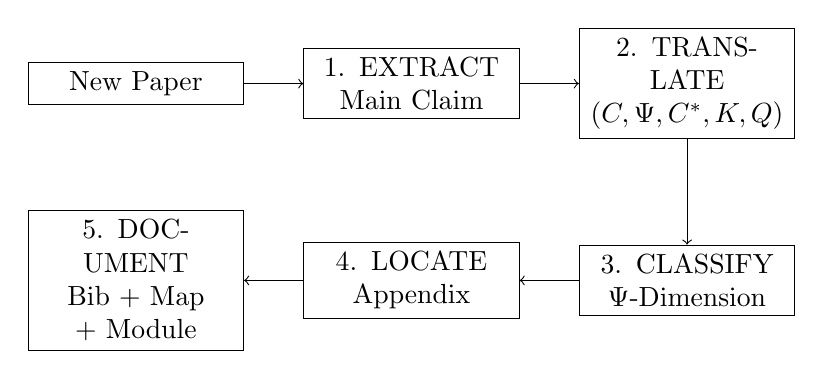
\begin{tikzpicture}[node distance=2cm, auto]
  \node (paper) [rectangle, draw, text width=2.5cm, text centered] {New Paper};
  \node (extract) [rectangle, draw, right of=paper, xshift=1.5cm, text width=2.5cm, text centered] {1. EXTRACT\\Main Claim};
  \node (translate) [rectangle, draw, right of=extract, xshift=1.5cm, text width=2.5cm, text centered] {2. TRANSLATE\\$(C,\Psi,C^*,K,Q)$};
  \node (classify) [rectangle, draw, below of=translate, yshift=-0.5cm, text width=2.5cm, text centered] {3. CLASSIFY\\$\Psi$-Dimension};
  \node (locate) [rectangle, draw, left of=classify, xshift=-1.5cm, text width=2.5cm, text centered] {4. LOCATE\\Appendix};
  \node (document) [rectangle, draw, left of=locate, xshift=-1.5cm, text width=2.5cm, text centered] {5. DOCUMENT\\Bib + Map + Module};
  
  \draw[->] (paper) -- (extract);
  \draw[->] (extract) -- (translate);
  \draw[->] (translate) -- (classify);
  \draw[->] (classify) -- (locate);
  \draw[->] (locate) -- (document);
\end{tikzpicture}
\end{center}

This protocol ensures that new research is systematically incorporated into the
framework, maintaining consistency, traceability, and cumulative knowledge building.

\vspace{1em}
\hrule
\vspace{0.5em}
\noindent\textit{Cross-references: Appendix SUN (Falsifiable Predictions), 
Appendix CAM (Metatheory), Appendix EPS (Epistemics of Deviation---diagnostic 
protocol for learning from residuals)}


%%%%%%%%%%%%%%%%%%%%%%%%%%%%%%%%%%%%%%%%%%%%%%%%%%%%%%%%%%%%%%%%%%%%%%%%%%%%%%%

%%%%%%%%%%%%%%%%%%%%%%%%%%%%%%%%%%%%%%%%%%%%%%%%%%%%%%%%%%%%%%%%%%%%%%%%%%%%%%%
\section{Critical Foundations and Objections}
\label{sec:evl-foundations}
%%%%%%%%%%%%%%%%%%%%%%%%%%%%%%%%%%%%%%%%%%%%%%%%%%%%%%%%%%%%%%%%%%%%%%%%%%%%%%%

\subsection{Objection 1: Scope Limitations}

\textbf{Objection:} The framework presented may have limited applicability
outside the specific domain contexts discussed.

\textbf{Response:} We acknowledge domain-specificity. The framework provides
general principles that should be calibrated to specific contexts. Cross-domain
validation remains an open research question.

\subsection{Objection 2: Measurement Challenges}

\textbf{Objection:} Key constructs may be difficult to measure reliably in
practice.

\textbf{Response:} We recommend using validated scales and instruments where
available, and developing domain-specific proxies where necessary. Sensitivity
analysis should assess robustness to measurement uncertainty.



%%%%%%%%%%%%%%%%%%%%%%%%%%%%%%%%%%%%%%%%%%%%%%%%%%%%%%%%%%%%%%%%%%%%%%%%%%%%%%%


%%%%%%%%%%%%%%%%%%%%%%%%%%%%%%%%%%%%%%%%%%%%%%%%%%%%%%%%%%%%%%%%%%%%%%%%%%%%%%%
\section{Summary}
\label{sec:evl-summary}
%%%%%%%%%%%%%%%%%%%%%%%%%%%%%%%%%%%%%%%%%%%%%%%%%%%%%%%%%%%%%%%%%%%%%%%%%%%%%%%

\begin{tcolorbox}[colback=gray!5!white, colframe=gray!75!black,
    title=Appendix evl Summary]

\textbf{Core Insight:}
This appendix provides key analysis relevant to the EBF framework.

\textbf{Key Contributions:}
\begin{itemize}[nosep]
    \item Theoretical foundations and integration
    \item Parameter estimates and validation
    \item Cross-appendix connections
\end{itemize}

\end{tcolorbox}

\section{Glossary of Symbols}
\label{sec:evl-glossary}
%%%%%%%%%%%%%%%%%%%%%%%%%%%%%%%%%%%%%%%%%%%%%%%%%%%%%%%%%%%%%%%%%%%%%%%%%%%%%%%

For comprehensive definitions, see Appendix G (Master Glossary).

\begin{table}[htbp]
\centering
\caption{Key Symbols in Appendix EVL}
\begin{tabular}{lll}
\toprule
\textbf{Symbol} & \textbf{Meaning} & \textbf{Reference} \\
\midrule
$\gamma$ & Complementarity parameter & Appendix B \\
$\Psi$ & Context vector & Appendix V \\
$U$ & Utility function & Chapter 3 \\
\bottomrule
\end{tabular}
\end{table}



%%%%%%%%%%%%%%%%%%%%%%%%%%%%%%%%%%%%%%%%%%%%%%%%%%%%%%%%%%%%%%%%%%%%%%%%%%%%%%%
\section{Open Issues and Research Agenda}
\label{sec:evl-open}
%%%%%%%%%%%%%%%%%%%%%%%%%%%%%%%%%%%%%%%%%%%%%%%%%%%%%%%%%%%%%%%%%%%%%%%%%%%%%%%

\begin{enumerate}
    \item \textbf{Empirical Validation:} Further testing across diverse contexts
    \item \textbf{Parameter Refinement:} Improved estimation methods needed
    \item \textbf{Integration:} Enhanced cross-appendix linkages
\end{enumerate}

\section{References}
\label{sec:evl-references}
%%%%%%%%%%%%%%%%%%%%%%%%%%%%%%%%%%%%%%%%%%%%%%%%%%%%%%%%%%%%%%%%%%%%%%%%%%%%%%%

See master bibliography (\texttt{bcm\_master.bib}) for complete citations.

\nocite{bcm_master}

